\documentclass{beamer}
\usetheme{LSUBeamer}
\setlength{\unitlength}{1in}

\usepackage[orientation=landscape,size=custom,width=48,height=36,scale=0.5,debug]{beamerposter}
\usepackage{graphicx}
\graphicspath{{./Figures/}}
\usepackage[absolute,overlay]{textpos}
\usepackage{amsmath}
\usepackage{siunitx}
\usepackage[export]{adjustbox}
\usepackage{tikz}
\usepackage{xcolor}
\usepackage{ragged2e}
\usepackage{mathrsfs}
\usepackage{array}
\usepackage{lmodern}
\usefonttheme{serif}
\usepackage{bm}
\usepackage{enumitem}
\usepackage{caption}
\usepackage{subcaption}
\usepackage{verbatim}
\usepackage{tabu}

\title{Embedded Development for Spaceflight Radiation Detectors}
\author{Duncan Wilkie, Jacob Miller, Jared Taylor, Jeffrey Chancellor}

\begin{document}
\begin{frame}
  \begin{columns}[t]
    \begin{column}{0.34\linewidth}
      \begin{block}{Abstract}
        Understanding the radiation environment inside a spacecraft is essential for safe long-term human occupation of space. Currently, detectors capable of tracking the highly energetic, massive particles encountered in cosmic rays are designed for ground-based operation, and present data in ways optimized for analysis by researchers. In this poster, efforts are showcased to develop an iOS-based interface with ADVACAM's Timepix detectors that allows for easy and user-friendly presentation of key information of medical interest, without compromising the quality of data gathered. Specifically, the resolution of challenges faced in embedded development of a communications channel between the Timepix output and Apple's proprietary iAP2 protocol are detailed. The development targets Texas Instruments Tiva C microcontrollers based on the ARM Cortex M4 architecture, and implements I2C, USB, and UART communication. Also presented is work on user interface design and low-bandwidth remote data transfer over iCloud, the integration of which is a major advantage of the design.
      \end{block}
      \begin{block}{The TM4C123}
        Ample timers, peripherals, clock modes, and bytes of flash memory led us to choose this ARM implementation.
\[        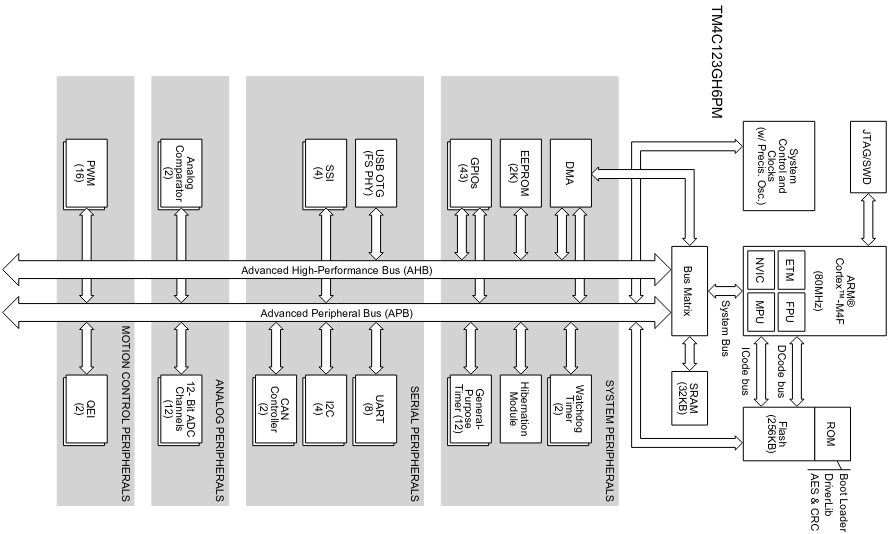
\includegraphics[scale=0.45, angle=90]{tm4c123blk.png}\]
      \end{block}


    \end{column}

    \begin{column}{0.38\linewidth}
      \begin{block}{Ergz iPad Application}
        The new iPad mini, with a \SI{96}{W} output rating, gets around the peak current problems with all other Apple devices and enables untethered operation. The interface allows quick reading of several relevant medical factors: instantaneous dose rate, total dose over selected time range, average dose rate over selected time range, and peak instantaneous dose. Development simulation captures appear below.
        \begin{figure}
          \centering
          \begin{subfigure}{.5\textwidth}
            \centering
            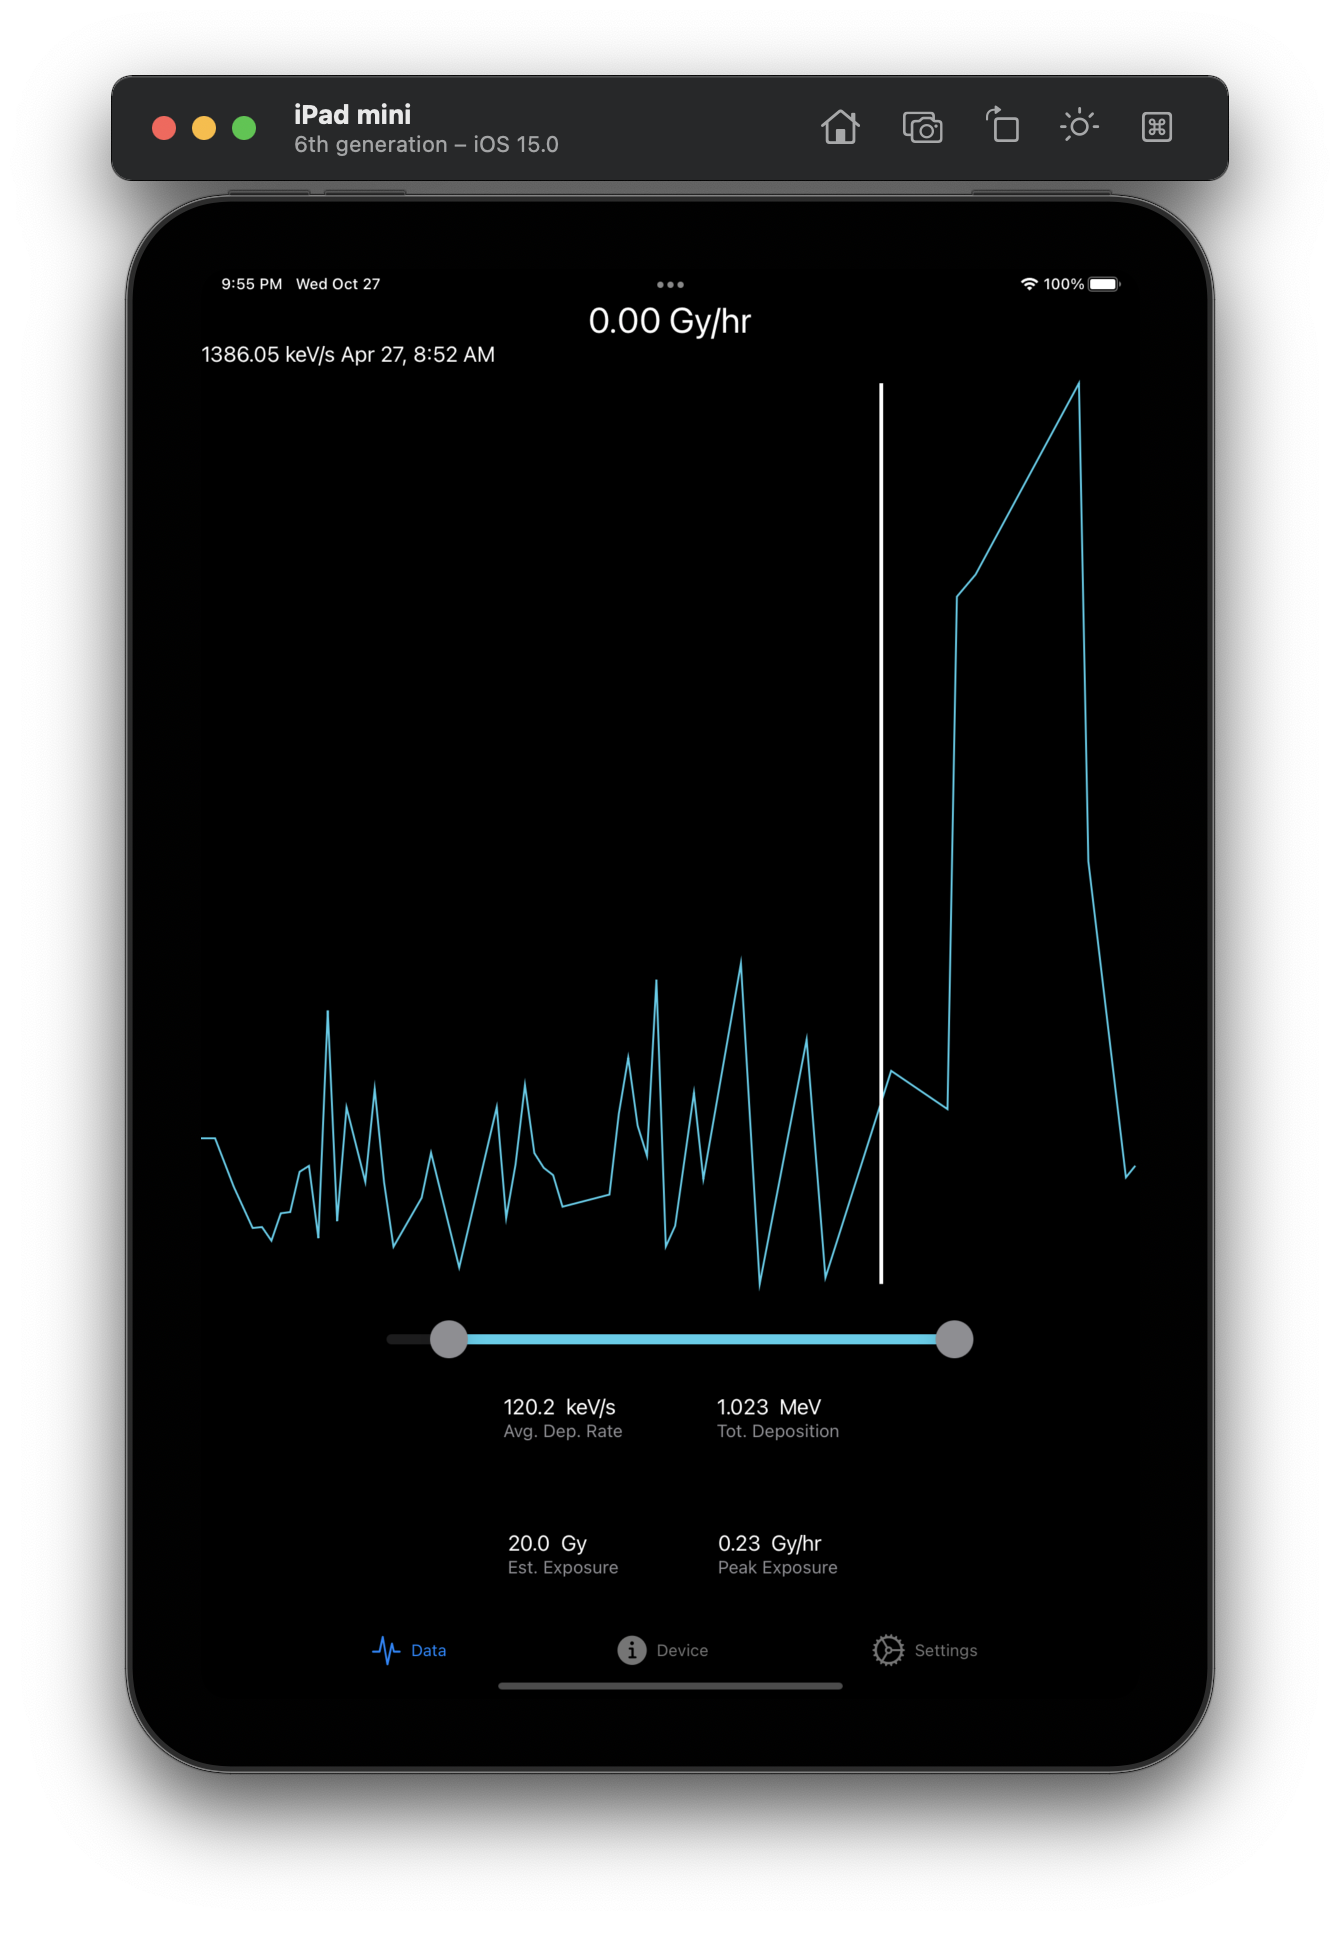
\includegraphics[width=.9\linewidth]{screen1.png}
            \caption{Medical Information}
          \end{subfigure}%
          \begin{subfigure}{.5\textwidth}
            \centering
            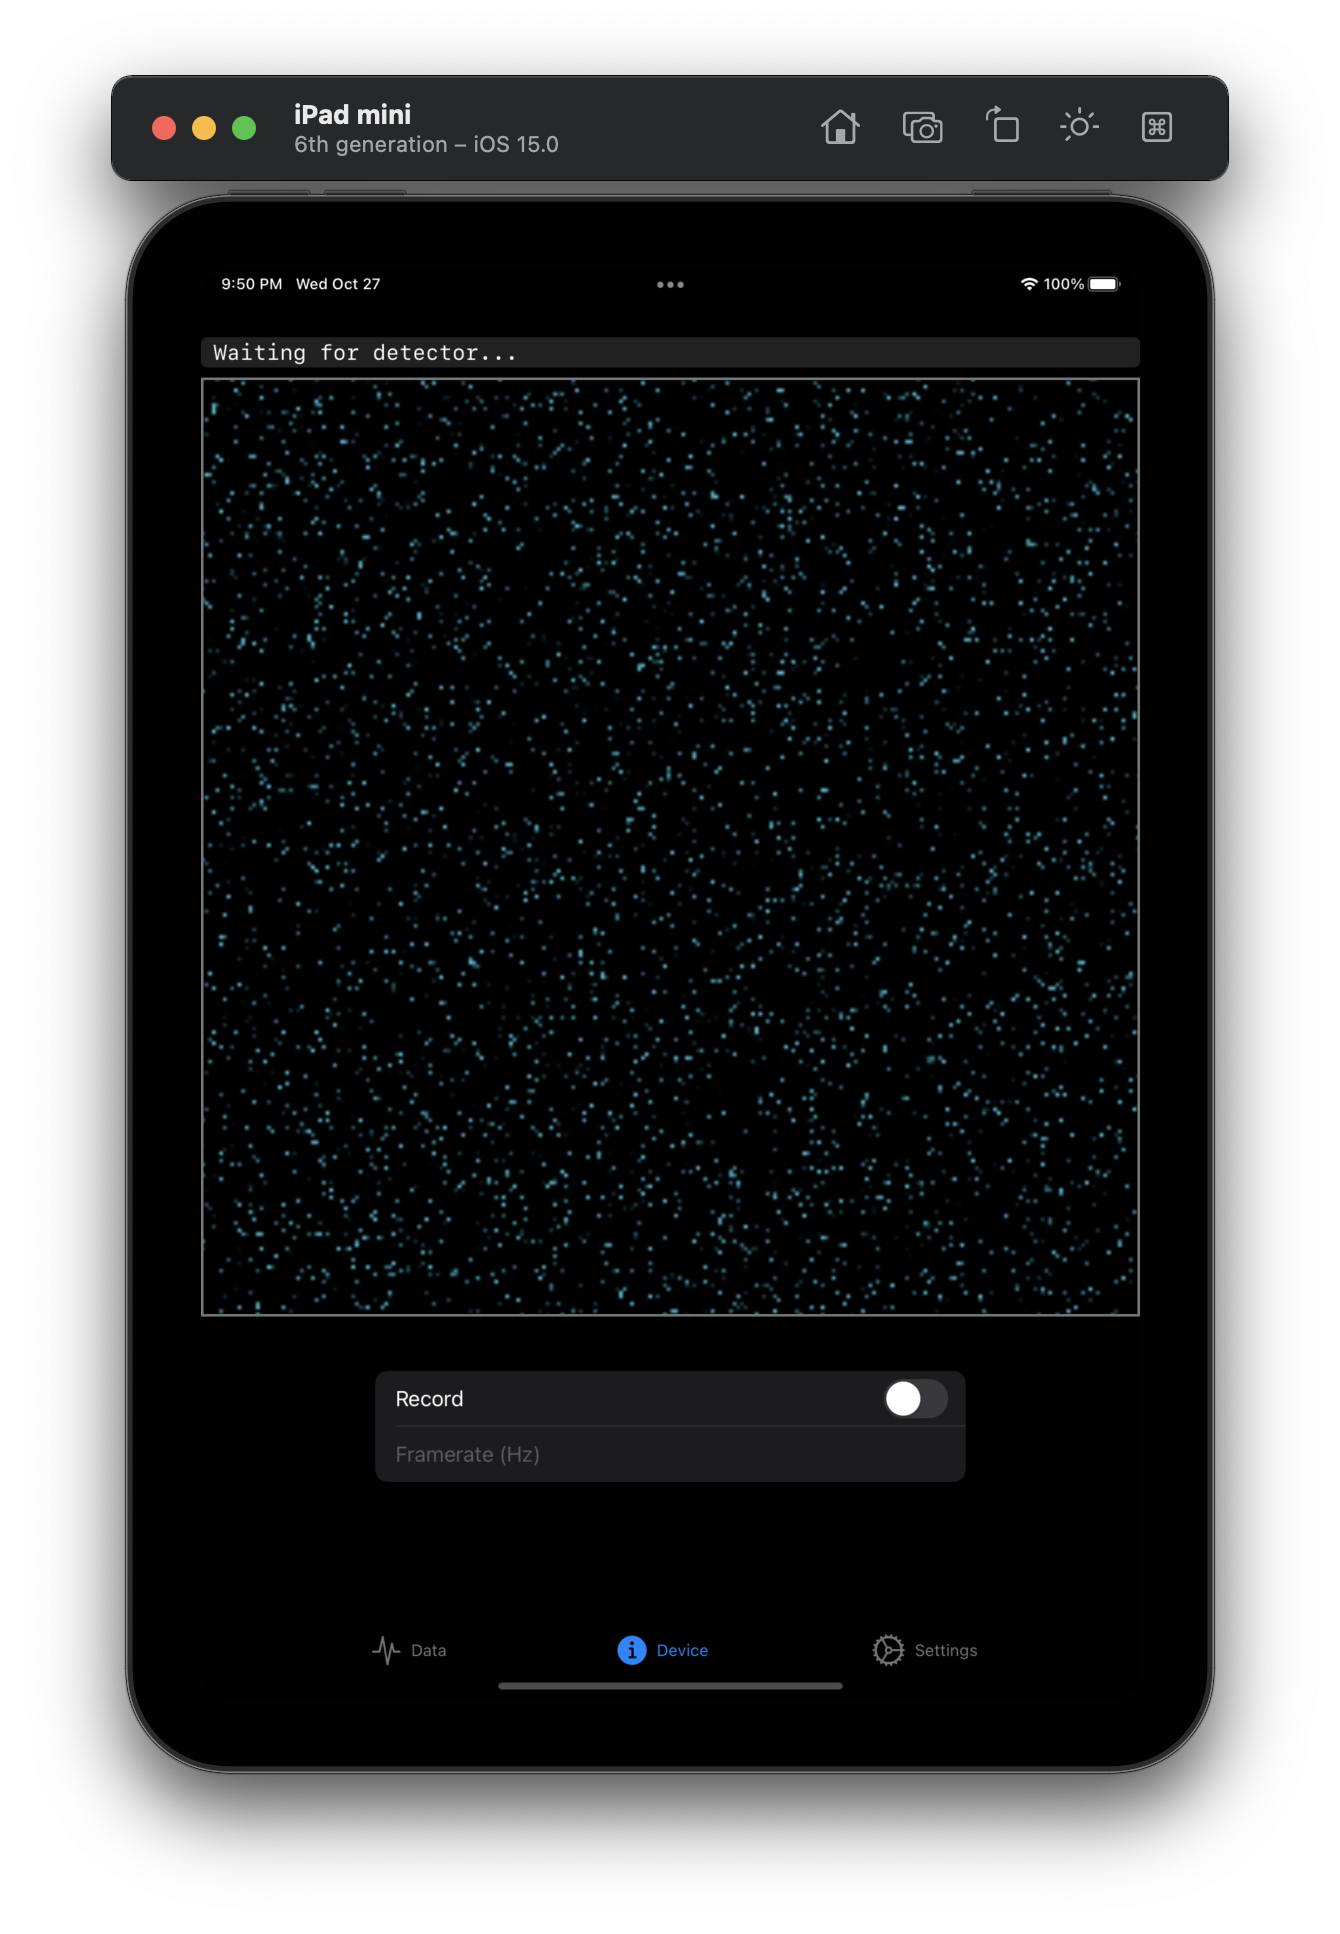
\includegraphics[width=.9\linewidth]{screen2.png}
            \caption{Detector Information}
          \end{subfigure}
        \end{figure}
      \end{block}
      \begin{block}{iCloud Integration}
        Ergz is able to back up its recorded data to the Apple iCloud. This enables remote interaction with data as it's collected. As an example of the value that provides, the following zsh script skeleton could be used on a stationary Mac server to produce a Web-exposed directory that can, for example, be accessed on-demand by higher caliber analysis tools such as CERN ROOT.
        \verbatiminput{autoscript.zsh}

      \end{block}
    \end{column}
    \begin{column}{0.24\linewidth}


      \begin{block}{Conclusion}

        The device developed as a result of this work promises to greatly expand the extent to which medical and medical physics professionals alike are able to easily record and analyze radiation environments, particularly space-based ones, and any associated health risks. In the near future, the results of this work will hopefully be available for use by those professionals.
      \end{block}

      \begin{block}{Acknowledgments}
        D.W. and J.C. acknowledge support from LaSPACE/NASA through grant 80NSSC20M0110. All of the authors acknowledge support from the Translational Research Institute for Space Health (TRISH) through the grant, (TREMS)/EXP0004 Timepix-based Radiation Environment Monitor for SpaceX. Additional assistance was provided by Jill Juneau of the Electronics Development Group, and the Machine Shop at .
      \end{block}
      \begin{block}{Affiliations}
        Duncan Wilkie: Department of Physics \& Astronomy and Department of Mathematics, Louisiana State University.
        Jacob Miller: Division of Electrical and Computer Engineering, Louisiana State University.
        Jared Taylor: Department of Physics \& Astronomy, Louisiana State University.
        Jeffery Chancellor:  Department of Physics \& Astronomy, Louisiana State University, Department of Preventive Medicine \& Population Health, UTMB, Outer Space Institute, University of British Columbia.

      \end{block}


    \end{column}
  \end{columns}
\end{frame}
\end{document}

%%% Local Variables:
%%% mode: latex
%%% TeX-master: t
%%% End:
